\renewcommand{\chaptername}{Protocolos de comunicación Serie}
%\graphicspath{{Apéndice/ComSPII2C/}}
\chapter{Protocolos de comunicación Serie}\label{AP:protSerial}
\section{Introducción}
En la presente sección, se describen dos protocolos utilizados con los periféricos seleccionados para el presente trabajo final. Los dos protocolos que utilizan estos dispositivos se denominan Serial Peripherical Interface o SPI, por sus siglas en inglés, y el protocolo I2C (también se lo puede encontrar con el nombre de Two Wire o TWI). Ambos protocolos definen señales de entrada y salida, y un dispositivo maestro, que es el encargado de enviar los datos a los periféricos correspondientes. En este trabajo, el dispositivo maestro, es el microcontrolador ATmega328P. Ambos protocolos son de tipo serie. Además, se revisa el pinout disponible de cada dispositivo, y se da una breve explicación sobre cada pin que poseen los perifericos (w5100 ethernet y display LCD con chip adaptador para I2C. 


\section{Protocolo SPI}

El protocolo SPI, define tres señales: MOSI,MISO y SCK o CLOCK. Dado que el protocolo SPI, consta de un dispositivo maestro, puede constar de varios dispositivos esclavos. Para seleccionar el dispositivo con el que se quiere comunicar, se debe agregar un cable adicional por dispositivo, este cable adicional se denomina Slave Select, o SS. El dispositivo maestro, selecciona un dispositivo esclavo para comunicarse a través de esta linea, denominada SS. A continuación, se deja una imagen de las conexiones entre un dispositivo maestro y tres esclavos: 

\begin{figure}[H]
	\centering	
	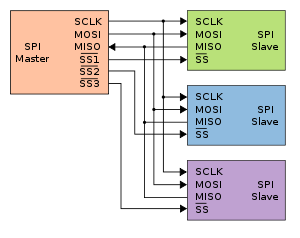
\includegraphics{Apéndice/ComSPII2C/SPIconn.png}
	\caption{Esquema de conexiones entre un dispositivo maestro y un dispositivo esclavo usando el protocolo SPI.}
	\label{fig:master_slave_SPI}
\end{figure}

Las señales que utiliza el protocolo SPI son las siguientes: 
\begin{itemize}
	\item SCK o CLOCK: Se encarga de generar una señal de reloj. Esta señal es generada por el dispositivo maestro.
	\item MOSI(Master Output Slave Input): Son los datos que envía el dispositivo maestro al esclavo. 
	\item MISO(Master Input Slave Output): Son los datos que envía el dispositivo esclavo al maestro. 
\end{itemize}

El dispositivo maestro, es el encargado de seleccionar a que dispositivo se quiere comunicar, mediante la línea o cable de SS en la figura \ref{fig:master_slave_SPI}. Además, el maestro, puede recibir información del dispositivo esclavo. Por tanto, la comunicación es de tipo ``full-duplex''(ambos dispositivos son capaces de transmitir y de recibir al mismo tiempo). Todos los datos salientes, se transmiten en serie, por ende, es requisito, que cada dispositivo maestro y/o esclavo, posean un registro de desplazamiento a medida que se reciben los datos.     
 
Esta comunicación es sincrónica, la señal de CLOCK, genera una señal de reloj,de una determinada frecuencia, y esta es utilizada para la sincronía con las señales MOSI y MISO respectivamente, para que se transfieran los datos entre sí. La señal de clock, solo esta activa durante la comunicación, luego se queda en estado alto o bajo, según se haya definido previamente. Debido a esto, se pueden definir cuatro modos de funcionamiento, dos basados en la polaridad del reloj, y otros dos, basados en la fase de la señal de reloj. En la siguiente imagen, se muestra un diagrama de tiempos de las señales involucradas en el protocolo SPI.  

\begin{figure}[ht]
	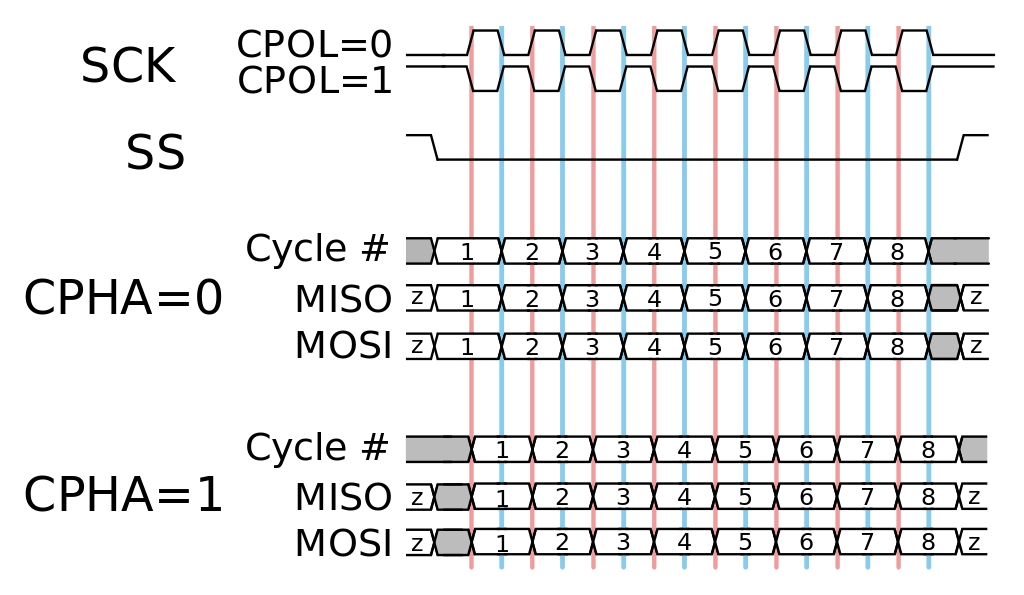
\includegraphics[width=\linewidth,height=8cm]{Apéndice/ComSPII2C/SPI_timing.png}
	\caption{Señales del protocolo SPI en función del tiempo. La letra z dentro del diagrama indica estado de alta impedancia}
	\label{fig:señales_SPI}
\end{figure}

Como se observa, en la figura, primero se pone la señal de slave select(ss) en nivel bajo, y luego empieza la comunicación. Cuando finaliza la comunicación, vuelve a su estado alto. Las señales se denominan CPOL por las siglas de ``clock polarity'' y CPHA por ``clock phase''. De la figura, se observa que hay cuatro modos de funcionamiento: 

\begin{itemize}
	\item Modo 0: Con CPOL = 0 y CPHA = 0. Modo en el cual el estado del reloj permanece en estado lógico bajo y la información se envía en cada transición de bajo a alto, es decir alto activo.
	\item Modo 1:CPOL=1 y CPHA = 1. El estado del lógico del reloj es alto, y se envían datos cuando hay una transición del estado alto al estado bajo. 
	\item Modo 2: CPOL = 1 y CPHA =0. El estado lógico del reloj es alto, y se envían los datos en cada transición de bajo a alto(existe un desfase entre el estado lógico y el envío de los datos).   
	\item Modo 3: CPOL = 1 y CPHA = 1. Modo en el cual el reloj permanece en estado lógico alto y la información se envía en cada transición de alto a bajo, es decir bajo activo.(existe un desfase entre el estado lógico y el envío de los datos). 
\end{itemize}

Por último, se debe destacar, que no todos los dispositivos soportan todos los modos, por ende, para realizar una comunicación entre dos dispositivos, se debe verificar que ambos por los menos tengan un modo en común para que la comunicación pueda llevarse a cabo. 



\section{Procotolo I2C}

El protocolo I2C, o Wire Serial, es un protocolo de comunicación serie, el cual define dos señales: SDA y SCL. La señal SDA es para transmitir los datos en formato serie(SDA proviene de las siglas serial data), y SCL, es una señal de reloj(SCL proviene de serial clock, en otras bibliografías, las puede encontrar como SCK o CLK). 

Este protocolo, presenta una arquitectura del tipo maestro esclavo. El maestro es el encargado de enviar los datos, y los reciben los esclavos. Puede existir más de un maestro. El diagrama eléctrico es el siguiente: 

\begin{figure}[ht]
	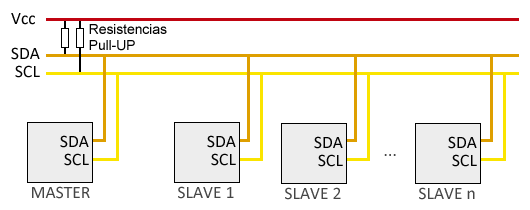
\includegraphics[scale=0.8]{Apéndice/ComSPII2C/busI2C.png}
	\caption{diagrama de las conexiones entre una maestro y n esclavos mediante el uso del protocolo I2C} 
	\label{fig:busI2C}
\end{figure}

Dado, que solo tiene dos cables, la forma de identificar un dispositivo es mediante una dirección, esta dirección, es un número binario formado por 7 bits, o 10 bits(en este último caso, son muy escasos los dispositivos), según el dispositivo. Si la dirección del esclavo, contienen solo 7 bits, esto quiere decir, que se puede conectar hasta 128 dispositivos. Esta dirección, debe ser dada por el fabricante del dispositivo o debe configurarse de alguna forma provista por el fabricante.  

El maestro, se comunica con los esclavos, mediante el uso de una secuencia de inicio, y una secuencia de parada, con esto, los esclavos reconocen si se quiere comunicar con alguno de ellos. Entre mensajes, existen bits de reconocimiento que el esclavo envía al maestro, para que el maestro pueda reconocer de qué forma se están recibiendo los datos por parte de los esclavos o esclavo correspondiente. 

\begin{figure}[ht]
	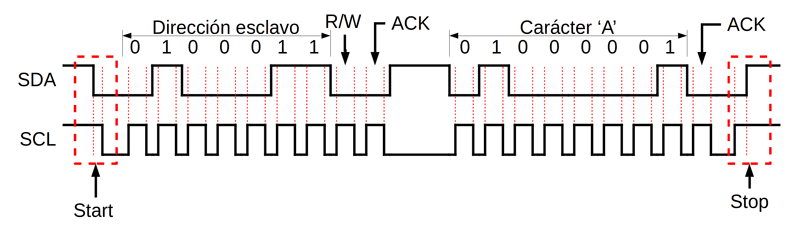
\includegraphics[scale=0.5]{Apéndice/ComSPII2C/timing_I2C.png}
	\caption{Diagrama de tiempos que utiliza el protocolo I2C.En este caso, se utiliza una dirección de 7 bits}
	\label{fig:timing_I2C}
\end{figure}

Como se observa en la figura \ref{fig:busI2C}, el estado del canal de comunicación por defecto es el estado alto. Cuando el master quiere iniciar la comunicación, pone la línea SDA en bajo, eso les indica a los esclavos que se va a iniciar una comunicación por parte del master. Acto seguido, se inicia la señal de SCL, la cual es una señal de reloj(ver figura \ref{fig:timing_I2C}). Luego se envían de forma sincronizada la dirección del esclavo con el cual se quiere comunicar, y un bit extra, el cual le avisa si requiere información del dispositivo o va a enviarle información. El dispositivo que posee esa dirección, reconoce que le van a enviar datos, y envía un bit de ACK, sobre la línea SDA, poniéndola en bajo. Luego, envía otros 8 bits, y el esclavo transmite un ACK, poniendo la linea SDA en bajo. Así, cada 8 bits, luego cuando la linea SCL permanece en alto, significa que la comunicación ha finalizado. Si el dispositivo no esta disponible, o no existe esa dirección, la señal SDA permanece en alto, y se corta la comunicación. Por otro lado, si la comunicación es del esclavo al maestro, el maestro también debe enviarle el bit de confirmación correspondiente.  

Cabe destacar, que la velocidad de comunicación viene dada por la señal de reloj. Se definen cuatro modos de velocidad para el bus I2C: 
\begin{itemize}
	\item MODO ESTANDAR
	\item MODO RAPIDO 
	\item MODO HIGH SPEED
	\item MODO ULTRA FAST 
\end{itemize}

Cada modo, define una frecuencia para su señal de reloj. Cuando se desean conectar maestros y esclavos, debe verificarse con su hoja de datos que ambos posean el mismo modo de velocidad, para cada dispositivo. 


\section{Chip ETHERNET W5100 shield }

El chip ethernet W5100, ya viene en un módulo integrado, mostrado en la figura \ref{fig:chip_ethernet}. Este módulo, posee 10 pines. Este módulo, trae un circuito integrado denominado W5100, el cual, se utiliza para proveer soluciones ethernet. Soporta los protocolos TCP/IP, y se puede configurar, para que se conecte a la red local mediante un cable ethernet. 

Los puertos que tiene este módulo son los siguientes(ver figura \ref{fig:ap_ethernet}):

\begin{itemize}
	\item pin Vcc: Pin donde se debe conectar una fuente de alimentación de 5Volts
	\item pin GND: Se conecta la tierra del sistema. 
	\item pin SS: Cable de slave select para el protocolo SPI 
	\item pin MOSI:Línea MOSI para el protocolo SPI  
	\item pin MISO Línea MISO para el protocolo SPI  
	\item pin SCK o CLOCK: Línea CLOCK para el protocolo SPI  
	\item pin Reset: Resetea el dispositivo ethernet, borrando todas sus configuraciones. 
	\item pin P+: Power of Ethernet. Cable destinado a recibir alimentación por la línea de red ethernet.Recibe potencia positiva 
	\item pin P+: Power of Ethernet. Cable destinado a recibir alimentación por la línea de red ethernet.Recibe potencia negativa  
\end{itemize}

Cabe destacar, que las lineas P+ y P-, son para poder utilizar el estandar "Power of Ethernet", el cual define lineas para la transmisión de la alimentación a través de un cable de red. 

\begin{figure}[ht]
	\centering 
	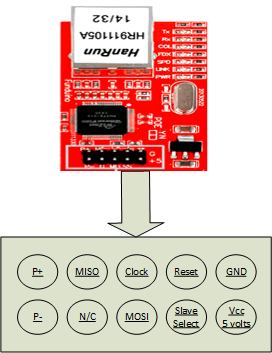
\includegraphics{parte_2/soft_micro/pinoutW5100}
	\caption{Esquema de pines que posee el módulo W5100.} 
	\label{fig:ap_ethernet}
\end{figure}

Si se observa la hoja de datos del dispositivo, se observan que los modos SPI soportados son los modos 0 y 3 respectivamente(véase pag. 61 de \cite{datsheetw5100}). 


\section{Display LCD con adaptador para I2C }

En el caso del display, el display, trae integrado un adaptador para I2C. Este adaptador es el circuito integrado PCF8574. Este según su hoja de datos(ver \cite{datsheetLCD}), se utiliza para expandir la cantidad de puertos de un microcontrolador, mediante el protocolo I2C a través de dos puertos, ya que este protocolo solo utiliza dos líneas para su comunicación. 

Este dispositivo, (PCF8574) puede usarse para leer los puertos a la salida, o para escribir los puertos a su salida. En este caso particular, esta placa con este circuito integrado, está realizada para aplicarla exclusivamente a los displays LCD, y se provee la librería para su uso con el display LCD. 

Para conocer la dirección de comunicación, se debe revisar la hoja de datos, y puede darse hasta 8 direcciones distintas, en base a los puertos del circuito integrado, denominados A0,A1,A2,por el fabricante. Estos puertos del circuito integrado PCF8574 se encuentran disponibles en la placa para ser modificados. La siguiente imagen muestra su ubicación en la placa: 

\begin{figure}[ht]
	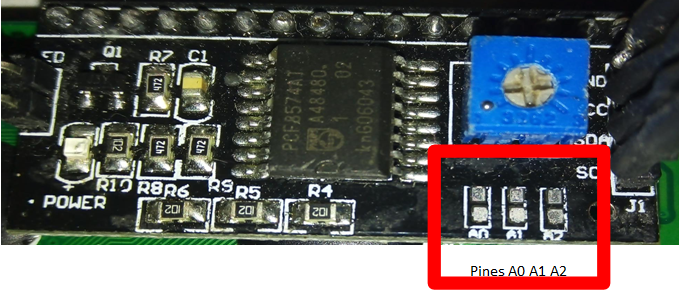
\includegraphics[scale=0.8]{Apéndice/ComSPII2C/display_LCDATRAS}
	\caption{Foto del display LCD de la parte de atrás, donde se observan los pines A0,A1 y A2 accesibles para poder modificarlos.}
	\label{fig:pcf8574_LCD} 
\end{figure}

Esta placa por defecto, trae todos los pines A0,A1 yA2 en alto. Si queremos pasar algún de esos puertos a bajo, se debe estaniar en donde se encuentra el cuadrado rojo en la imagen \ref{fig:pcf8574_LCD}. De la hoja de datos(pág. 13 de \cite{datsheetLCD}), se explica que la dirección posee 7 bits, donde los siete bits vienen dados en la forma 0100A2A1A0, si A0,A1 o A2 esta en alto, se indica un uno, caso contrario, se completa con cero. Por ejemplo si consideramos el caso de la figura, no ha sido modificado, por ende, A2 = 1 , A1 = 1 y A0 = 1. Esto nos indica que el dispositivo tiene la dirección 0100111, que es 27 en base hexadecimal. 

Entonces, este procedimiento de poder cambiar la dirección del puerto I2C, permite conectar hasta 8 chips iguales, obteniendo 64 puertos de entrada y salida, manejado únicamente desde un dispositivo maestro, a través de dos líneas. Esto claramente presenta la ventaja de requerir menor cantidad de puertos, que un display LCD, y la diferencia de precios entre un display LCD, con chip I2C es ínfima, y no conviene optar por el display LCD sin el chip(la diferencia en pesos argentinos ronda los \$200,en esta época,esto equivale a 1,25 dólares aproximadamente al escribir esta sección del presente documento). 

Los puertos que tiene disponibles a la salida, son Vcc Y GND. En el pin de Vcc deben conectarse 5 volts, y en GND la tierra. Los puertos SDA y SCL, son los puertos del protocolo I2C, y se deben conectar como en la figura \ref{fig:busI2C}. En el caso, de conectarla a la placa Arduino Uno, como en este caso, las resistencias de pull-up, están implementadas sobre la misma placa. 
